\subsubsection{Thiết kế Sitemap}

\begin{figure}[H]
    \centering
    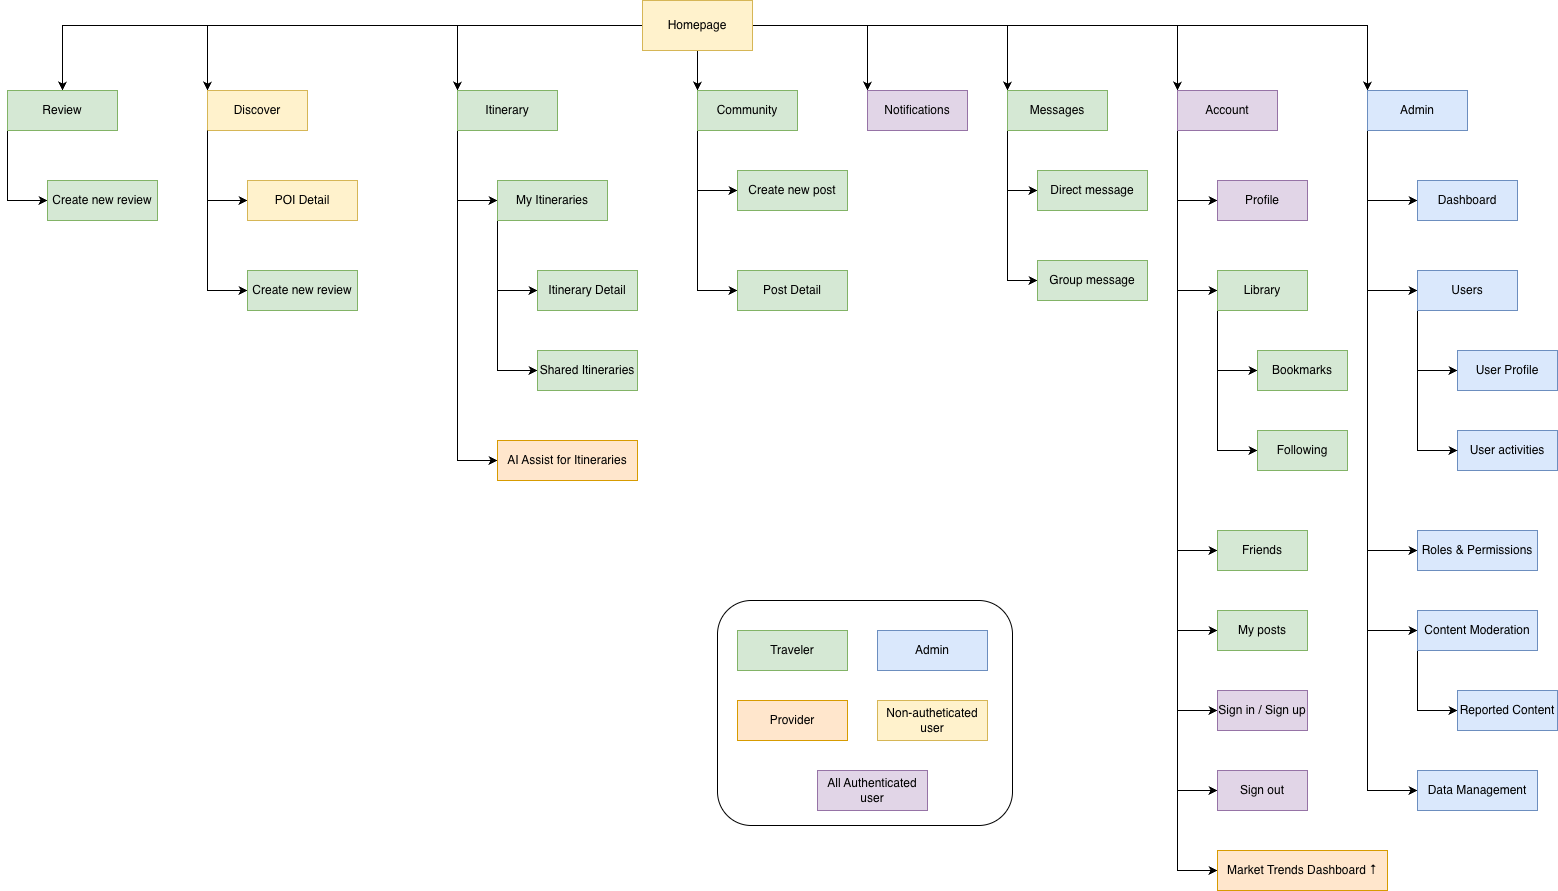
\includegraphics[width=1\textwidth]{Images/7. System Design/Sitemap.png}
    \caption{Sitemap của hệ thống TravelEZ}
    \label{fig:sitemap}
\end{figure}

Sitemap này mô tả cấu trúc và các tính năng chính của Hệ thống TravelEZ, nêu chi tiết các chức năng và mô-đun cốt lõi của nó. Dưới đây là bảng tóm tắt các trang chính và mục đích của chúng trong hệ thống:
\begin{table}[H]
\centering
\begin{tabular}{|p{5cm}|p{10cm}|}
\hline
Page             & Mục đích                                                     \\ \hline
Trang chủ (Home) & Điểm vào hệ thống, điều hướng đến các chức năng chính.       \\ \hline
Explore          & Khám phá địa điểm và nội dung công khai.                     \\ \hline
POI Detail       & Xem chi tiết thông tin địa điểm (mô tả, hình ảnh, đánh giá). \\ \hline
\end{tabular}
\caption{Sitemap dành cho tất cả người dùng}
\label{tab:all-user}
\end{table}

\begin{table}[H]
\centering
\begin{tabular}{|p{5cm}|p{10cm}|}
\hline
Page                      & Mục đích                                                                         \\ \hline
Market Trends Dashboard   & Xem thống kê xu hướng điểm đến và nhu cầu dịch vụ để cải thiện sản phẩm/dịch vụ. \\ \hline
AI Assist for Itineraries & Gửi hành trình và nhận phân tích + đề xuất cải thiện từ AI.                      \\ \hline
\end{tabular}
\caption{Sitemap dành cho Nhà cung cấp (Provider)}
\label{tab:provider}
\end{table}

\begin{table}[H]
\centering
\begin{tabular}{|p{5cm}|p{10cm}|}
\hline
Page                & Mục đích                                                \\ \hline
Itinerary           & Quản lý và tạo hành trình cá nhân.                      \\ \hline
Recommendation      & Nhận hành trình đề xuất tự động theo sở thích.          \\ \hline
My Itineraries      & Danh sách hành trình của người dùng.                    \\ \hline
Itinerary Detail    & Xem chi tiết từng hành trình.                           \\ \hline
Shared Itineraries  & Xem các hành trình được chia sẻ công khai.              \\ \hline
Community           & Xem và tương tác với nội dung cộng đồng.                \\ \hline
Post Detail         & Xem chi tiết bài viết của người dùng khác.              \\ \hline
Review Detail       & Xem chi tiết bài đánh giá.                              \\ \hline
Create new post     & Tạo bài viết chia sẻ.                                   \\ \hline
Create new review   & Tạo đánh giá về địa điểm/dịch vụ.                       \\ \hline
Notifications       & Xem thông báo từ hệ thống.                              \\ \hline
Messages            & Trung tâm nhắn tin.                                     \\ \hline
Direct message      & Chat 1–1 với người dùng khác.                           \\ \hline
Group message       & Trò chuyện trong nhóm.                                  \\ \hline
Account             & Quản lý thông tin cá nhân \& hoạt động.                 \\ \hline
Profile             & Thông tin cá nhân.                                      \\ \hline
Library → Bookmarks & Quản lý bài viết/địa điểm đã lưu.                       \\ \hline
Library → Following & Xem danh sách chủ đề/địa điểm/người dùng đang theo dõi. \\ \hline
Friends             & Danh sách bạn bè, yêu cầu kết bạn.                      \\ \hline
Settings            & Thiết lập tài khoản cá nhân.                            \\ \hline
My posts            & Xem danh sách bài viết đã tạo.                          \\ \hline
My activities       & Xem và theo dõi các hoạt động (bình luận, review…).     \\ \hline
Sign in / Sign up   & Đăng nhập / Đăng ký tài khoản.                          \\ \hline
Sign out            & Đăng xuất khỏi hệ thống.                                \\ \hline
\end{tabular}
\caption{Sitemap dành cho Khách du lịch (Travelers) và người dùng đã xác thực.}
\label{tab:travelers}
\end{table}

\begin{table}[H]
\centering
\begin{tabular}{|p{5cm}|p{10cm}|}
\hline
Page                 & Mục đích                                             \\ \hline
Admin                & Khu quản trị hệ thống.                               \\ \hline
Dashboard            & Tổng quan dữ liệu (người dùng, nội dung, hoạt động). \\ \hline
Users                & Danh sách tài khoản.                                 \\ \hline
User Profile         & Xem thông tin của một người dùng.                    \\ \hline
User activities      & Xem lịch sử hoạt động của người dùng.                \\ \hline
Roles \& Permissions & Quản lý phân quyền.                                  \\ \hline
Content Moderation   & Xử lý báo cáo và kiểm duyệt nội dung.                \\ \hline
Reported Content     & Danh sách nội dung bị báo cáo vi phạm.               \\ \hline
Data Management      & Quản lý và xử lý dữ liệu hệ thống.                   \\ \hline
\end{tabular}
\caption{Sitemap dành cho Quản trị viên hệ thống (Admin)}
\label{tab:admin}
\end{table}

